\let\negmedspace\undefined
\let\negthickspace\undefined
\documentclass[journal]{IEEEtran}
\usepackage[a5paper, margin=10mm, onecolumn]{geometry}
%\usepackage{lmodern} % Ensure lmodern is loaded for pdflatex
\usepackage{tfrupee} % Include tfrupee package

\setlength{\headheight}{1cm} % Set the height of the header box
\setlength{\headsep}{0mm}  % Set the distance between the header box and the top of the text

\usepackage{gvv-book}
\usepackage{gvv}
\usepackage{cite}
\usepackage{amsmath,amssymb,amsfonts,amsthm}
\usepackage{algorithmic}
\usepackage{graphicx}
\usepackage{textcomp}
\usepackage{xcolor}
\usepackage{txfonts}
\usepackage{listings}
\usepackage{enumitem}
\usepackage{mathtools}
\usepackage{gensymb}
\usepackage{comment}
\usepackage[breaklinks=true]{hyperref}
\usepackage{tkz-euclide} 
\usepackage{listings}
% \usepackage{gvv}                                        
\def\inputGnumericTable{}                                 
\usepackage[latin1]{inputenc}                                
\usepackage{color}                                            
\usepackage{array}                                            
\usepackage{longtable}                                       
\usepackage{calc}                                             
\usepackage{multirow}                                         
\usepackage{hhline}                                           
\usepackage{ifthen}                                           
\usepackage{lscape}
\begin{document}

\bibliographystyle{IEEEtran}
\vspace{3cm}

\title{3.2.30}
\author{EE24BTECH11021 - Eshan Ray}

% \maketitle
% \newpage
% \bigskip
{\let\newpage\relax\maketitle}

\renewcommand{\thefigure}{\theenumi}
\renewcommand{\thetable}{\theenumi}
\setlength{\intextsep}{10pt} % Space between text and floats




\textbf{Question: }\\
Draw a parallelogram $ABCD$ in which $BC = 5 cm$, $AB = 3 cm$ and $\angle ABC = 60\degree$,
divide it into triangles $ACB$ and $ABD$ by the diagonal $BD$. Construct the triangle
$BD'C'$ similar to $\triangle BDC$ with scale factor $\frac{4}{3}$ . Draw the line segment $D'A'$ parallel to
$DA$ where $A'$ lies on extended side $BA$. Is $A'BC'D'$ a parallelogram?\\
\solution { 
\begin{table}[h!]    
  \centering
  \begin{tabular}[12pt]{ |c| c|}
    \hline
        \textbf{Variable}  & \textbf{Description} \\
    \hline
        $\vec{B}$$\brak{-4,0}$ &  coordinates of first point  \\
    \hline 
        $\vec{C}$$\brak{10,0}$ & coordinates of second point \\
    \hline
        $\vec{A}$& Equidistant point of $\vec{B}$ and $\vec{C}$ on $X$ axis \\  
    \hline
         
\end{tabular}

  \caption{Input parameters}
  \label{tab1.1.9.2}
\end{table}


\begin{figure}[!ht]
    \centering
	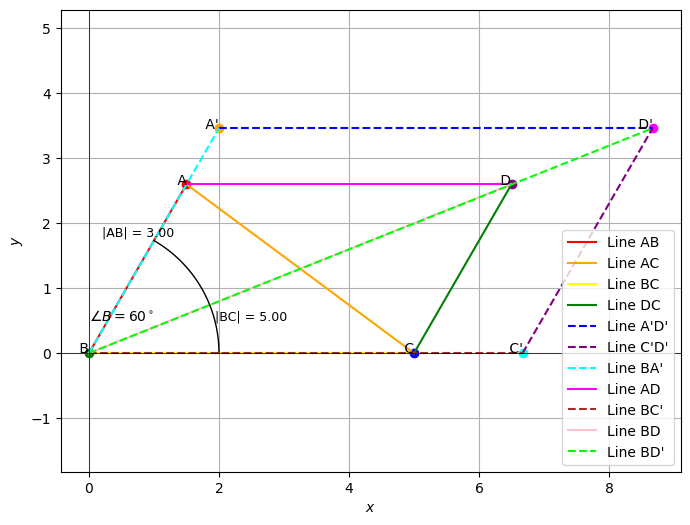
\includegraphics[width=1\textwidth]{plots/plot.png}
    \caption{$||^{gm} ABCD$ and $||^{gm} A'BC'D'$}
    \label{fig:plot}
\end{figure}  
\\
\\
\\

$ABCD$ is a parallelogram,
\begin{align}
\implies AB\parallel DC, AB&=DC\\
\implies AD\parallel BC, AD&=BC\\
  \triangle BDC\sim \triangle BD'C'\brak{Given}\\
     scale factor=\frac{4}{3}\\
         \implies \frac{BD'}{BD}&=\frac{4}{3}\\
         \implies \frac{BC'}{BC}&=\frac{4}{3}\\
         \implies \angle BCD &=\angle BC'D'\\
        \implies \angle BDC&=\angle BD'C'\\
        \therefore CD\parallel C'D'\\
BC'\parallel BC\\
         Given, $A'D'\parallel AD$\\
              From \triangle BA'D' & \triangle BAD,\\
         \implies \angle ABD&=\angle A'BD'\\
         \implies \angle BDA&=\angle BD'A'\\
         \implies \angle BAD&=\angle BA'D'
     \end{align}
     $\therefore \triangle ABD\sim \triangle A'BD'$
     \begin{align}
         \implies \frac{BD'}{BD}=\frac{BA'}{BA}=\frac{A'D'}{AD}=\frac{4}{3}
     \end{align}
     In quadrilateral $A'BC'D'$,
     \begin{align}
         A'D'\parallel AD\parallel BC\\
         \implies A'D'\parallel BC'\\
        \implies BC'&=\frac{4}{3}BC\\ \implies A'D'&=\frac{4}{3}AD\\
         \therefore BC'&=A'D'\\
         Similarly, BA'\parallel C'D', BA'= C'D'
     \end{align}
    So, quadrilateral $A'BC'D'$ is a parallelogram.
   }
\end{document}


